\documentclass{utils/BachelorBUI}

\usepackage[utf8]{inputenc}
\RequirePackage[babel,austrian=quotes,english=american]{csquotes}

\raggedbottom

\lstset{
    language={Matlab},
}

\sisetup{output-decimal-marker = {,},
    range-phrase = --,
    group-separator = {~},
    per-mode = symbol,
    list-final-separator={ und }}

\graphicspath{{images/}}

\newcommand{\zB}{\mbox{z.\,B.}\xspace}
\newcommand{\Name}[1]{\textsc{#1}}

\newcommand{\vKTxv}{\mathbf{v}_1^T\tilde{\mathbf{K}}_{T},_{\xi}\mathbf{v}_1}
\newcommand{\vKTxxv}{\mathbf{v}_1^T\tilde{\mathbf{K}}_{T},_{\xi\xi}\mathbf{v}_1}

\usepackage[style=numeric-comp,backend=biber,maxcitenames=2]{biblatex}
\ExecuteBibliographyOptions{%
    giveninits=true,maxbibnames=99}%
\DefineBibliographyStrings{english}{%
    andothers={et\;al\adddot},
    urlseen = {Zugriff am}
}
\addbibresource{utils/literature.bib}

\usepackage{acro}
\acsetup{list/display=used}

\usepackage{eurosym}

\DeclareAcronym{obv}{
short = {\"obv},
long  = {Österreichische Bautechnikvereinigung},
}

\DeclareAcronym{LZKB}{
short = {LZKB},
long  = {Lebenszykluskosten Brücken},
}

\DeclareAcronym{dt}{
short = {dt.},
long  = {deutsch},
}

\DeclareAcronym{abbv}{
short = {ABBV},
long  = {Ablösungsbeträge-Berechnungsverordnung},
short-plural = {s},
long-plural = {en},
}

\DeclareAcronym{lzk}{
short = {LZK},
long  = {Lebenszykluskosten},
extra = {[\officialeuro{}]},
}



\setcounter{biburllcpenalty}{9000}
\setcounter{biburlucpenalty}{9000}
\title{Schema-First Design in Web Apps: Integrating Angular, JsonForms and Spring Boot}
\authorname{Vlad-Ioan Dancea}
\email{danceavlad@icloud.com}
\MatrNr{12123455}
\thesislanguage{en-US}                        %% (de-AT, de-DE, en-GB, en-US)
\keywords{bachelor thesis\sep template\sep LaTeX}

\begin{document}

    \selectlanguage{english}

    \begin{filecontents}[overwrite]{\jobname.xmpdata}
        \makeatletter
        \Title{\@title}
        \Author{\@authorname}
        \Language{\@thesislanguage}
        \Keywords{\@keywords}
        \Publisher{TU Wien}
        \makeatother
    \end{filecontents}

    \maketitle

    %%%%%%%%%%%%%%%% Examples %%%%%%%%%%%%%%
    % Citation
    % \cite{Alberty:1999}

    % Footnote
    % \footnote{This is a footnote.}

    % Equation
    % \begin{equation}
    K_t
    =
    \left(
        1-
        \frac{R^2\cdot\tau}{c_a+\nu\cdot\tan\delta}
    \right)^4 \cdot k_1
    \label{Glg:Kt}
\end{equation}

    % Graphic
    % \usepackage{graphicx}
\begin{figure}[h]
    \centering{
        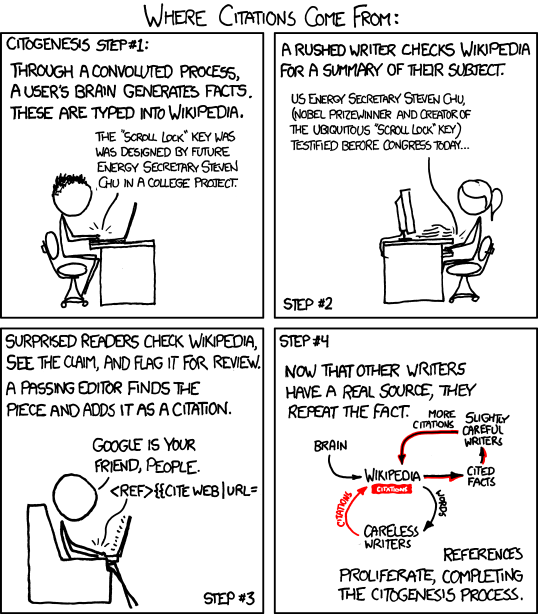
\includegraphics[width=9cm]{../images/citogenesis}
    }
    \caption{This is an example of a graphic}
    \label{fig:label:example-graphic}
\end{figure}

    % Table
    % \begin{table}[ht]
    \caption{The description comes above the table.
    Needs to be numbered.
    Last sentence without punctuation \label{tab:1}}
    \centering
    \begin{tabular}{lll}
        \toprule
        Column title 1 & Column title 2 & Column title 3 \\
        \midrule
        1  & 2  & 3  \\
        4  & 5  & 6  \\
        7  & 8  & 9  \\
        10 & 11 & 12 \\
        \bottomrule
    \end{tabular}
\end{table}

    % Code
    % \usepackage{listings}

\begin{lstlisting}[firstnumber=1,caption={Short caption},label={label}]
%FEM2D two-dimensional finite element method for Laplacian.
% Initialisation
load coordinates.dat; coordinates(:,1)=[];
eval('load elements3.dat; elements3(:,1)=[];','elements3=[];');
eval('load elements4.dat; elements4(:,1)=[];','elements4=[];');
eval('load neumann.dat; neumann(:,1) = [];','neumann=[];');
load dirichlet.dat; dirichlet(:,1) = [];
FreeNodes=@setdiff@(1:size(coordinates,1),unique(dirichlet));
A = sparse(size(coordinates,1),size(coordinates,1));
b = sparse(size(coordinates,1),1);

% Assembly
for j = 1:size(elements3,1)
  A(elements3(j,:),elements3(j,:)) = A(elements3(j,:),elements3(j,:)) ...
      + stima3(coordinates(elements3(j,:),:));
end
for j = 1:size(elements4,1)
  A(elements4(j,:),elements4(j,:)) = A(elements4(j,:),elements4(j,:)) ...
      + stima4(coordinates(elements4(j,:),:));
end
\end{lstlisting}
    %%%%%%%%%%%%%%%%%%%%%%%%%%%%%%%%%%%%%%%%

    \begin{abstract}
    Here comes the abstract of the thesis.
    It should be a short summary of the content of the thesis.
    It should contain at least 70 and at most 150 words.
    The font size should be 10pt.
    The left and right margins should be 1cm.
    The text in the abstract is written within the environment
    \texttt{\textbackslash{}begin\{abstract\}} and
    \texttt{\textbackslash{}end\{abstract\}}.
\end{abstract}

    \tableofcontents
    
    \section{Introduction}

The length of the Bachelor thesis is between 12 and 30 pages (excluding appendix).
After the title of the thesis, the author and a short abstract are given.
Then the main part of the thesis begins.
The Bachelor thesis has no title page and only an optional table of contents
(between abstract and chapter~1).

    \printbibliography

\end{document}